\documentclass[11pt]{article}

\usepackage[margin=0.95in]{geometry}
\usepackage{amsmath,amssymb}
\usepackage{microtype}
\usepackage{booktabs}
\usepackage{longtable}
\usepackage[svgnames,table]{xcolor}
\usepackage{tikz}
\usetikzlibrary{
  arrows.meta,
  positioning,
  shapes.geometric,
  shapes.misc,
  fit,
  backgrounds,
  calc,
  decorations.pathreplacing,
}
\usepackage{hyperref}
\hypersetup{colorlinks=true,linkcolor=Sienna,urlcolor=SteelBlue,citecolor=Sienna}
\usepackage{url}
\DeclareUrlCommand\fname{\urlstyle{tt}}

\setlength{\parindent}{0pt}
\setlength{\parskip}{0.55em}

%==============================================================
% Color palette
%==============================================================
\definecolor{solverCol}{HTML}{1F4E79}     % deep blue (solver / production)
\definecolor{solverBg}{HTML}{E7EEF6}
\definecolor{phaseA}{HTML}{0E7C7B}         % teal (Phase 6α)
\definecolor{phaseABg}{HTML}{E0F1F1}
\definecolor{phaseB}{HTML}{6A1B9A}         % purple (Phase 6β)
\definecolor{phaseBBg}{HTML}{F1E6F7}
\definecolor{deck}{HTML}{B7202C}           % red (deck / experiment)
\definecolor{deckBg}{HTML}{FBE5E7}
\definecolor{verdict}{HTML}{C77700}        % amber (verdict / blocker)
\definecolor{verdictBg}{HTML}{FFF3D9}
\definecolor{neutralCol}{HTML}{455A64}     % slate (neutral / context)
\definecolor{neutralBg}{HTML}{ECEFF1}
\definecolor{success}{HTML}{2E7D32}
\definecolor{badgegray}{HTML}{616161}

\tikzset{
  bigbox/.style={
    rectangle, rounded corners=6pt, line width=1.1pt, inner sep=10pt,
    align=left, font=\normalsize,
  },
  callout/.style 2 args={
    rectangle, rounded corners=5pt, draw=#1, line width=1pt,
    fill=#2, inner sep=8pt, align=left,
  },
  arrowBig/.style={
    -{Latex[length=3mm,width=2.5mm]}, line width=1.2pt, draw=black!55,
  },
  arrowMed/.style={
    -{Latex[length=2.5mm,width=2mm]}, line width=0.9pt, draw=black!55,
  },
}

%==============================================================
\title{\bfseries Phase 6$\alpha$ / Phase 6$\beta$:
       Closing the Selectivity Gap\\[2pt]
       \large{\normalfont Overview of the missing-physics investigation,
       May 2026}}
\author{\normalsize PNPInverse / Forward solver}
\date{\today}

\begin{document}
\maketitle

\begin{abstract}\noindent
Light-detail overview of the Phase 6$\alpha$ / Phase 6$\beta$ work.
The production PNP+BV forward stack converges across the deck's
voltage band and produces sensible Levich currents, but its H$_2$O$_2$
selectivity is flat across $V_{\mathrm{RHE}}$, while the Mangan/Seitz
deck data shows a distinct cathodic peak.  Phase 6$\alpha$ and 6$\beta$
are two hypotheses about what missing physics puts that peak there.
6$\alpha$ tested water self-ionization (retired as sub-leading).
6$\beta$ tested cation hydrolysis at the outer Helmholtz plane
following the group's own framing.  The 6$\beta$ architecture and
calibration landed cleanly; the fit step (10) hit a
non-identifiability verdict and is currently blocked.  This document
is the short story --- see the per-step handoffs in
\texttt{docs/phase6/} for the long ones.
\end{abstract}

\vspace{-0.4em}\hrule\vspace{0.4em}

%==============================================================
\section{The selectivity gap}
%==============================================================

The production solver and the deck disagree about one thing in a
specific way.  Both are at K$_2$SO$_4$, pH 4--6, $L_{\mathrm{eff}}
\approx 100~\mu$m, $V_{\mathrm{RHE}}$ in roughly $[-0.4, +0.55]$~V.
The solver's total disk current density matches the deck's order of
magnitude (Levich-limited cathodic), but the partial H$_2$O$_2$
current behaves differently:

\begin{center}
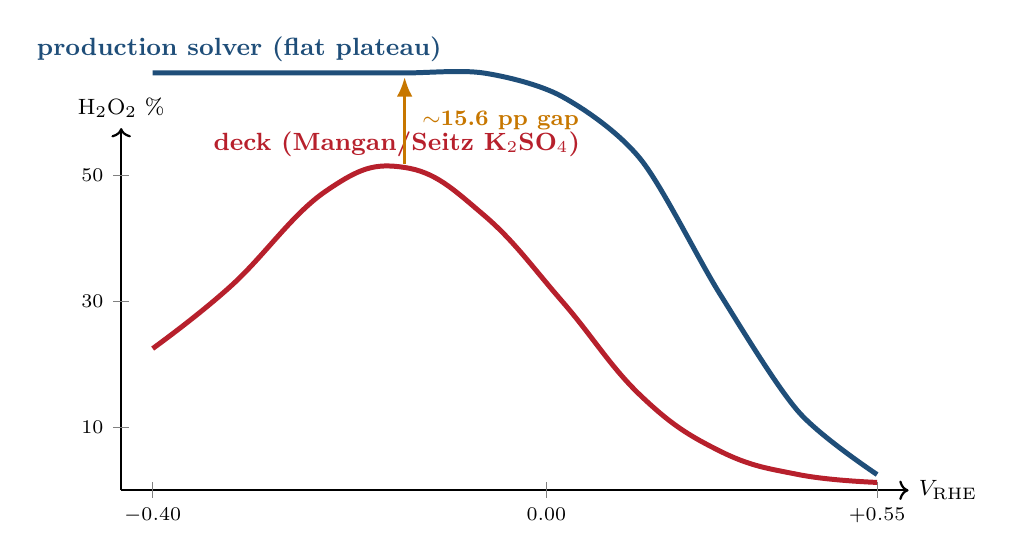
\begin{tikzpicture}[scale=1.0]

% Axes
\draw[->, line width=0.8pt] (0,0) -- (10,0) node[right, font=\footnotesize] {$V_{\mathrm{RHE}}$};
\draw[->, line width=0.8pt] (0,0) -- (0,4.6) node[above, font=\footnotesize] {H$_2$O$_2$ \%};

% X-axis ticks
\draw[draw=black!50] (0.4, 0.1) -- (0.4, -0.1) node[below, font=\scriptsize] {$-0.40$};
\draw[draw=black!50] (5.4, 0.1) -- (5.4, -0.1) node[below, font=\scriptsize] {$0.00$};
\draw[draw=black!50] (9.6, 0.1) -- (9.6, -0.1) node[below, font=\scriptsize] {$+0.55$};

% Y-axis ticks
\foreach \y/\lab in {0.8/10, 2.4/30, 4.0/50}
  \draw[draw=black!50] (-0.1, \y) -- (0.1, \y) node[left, font=\scriptsize] at (-0.1, \y) {\lab};

% Deck curve (with cathodic peak)
\draw[line width=1.8pt, draw=deck] plot[smooth, tension=0.7] coordinates
  {(0.4, 1.8) (1.4, 2.6) (2.6, 3.8) (3.6, 4.1) (4.6, 3.5) (5.6, 2.4) (6.6, 1.2) (7.6, 0.5) (8.6, 0.2) (9.6, 0.1)};
\node[deck, font=\small\bfseries] at (3.5, 4.4) {deck (Mangan/Seitz K$_2$SO$_4$)};

% Model curve (flat plateau)
\draw[line width=1.8pt, draw=solverCol] plot[smooth, tension=0.5] coordinates
  {(0.4, 5.3) (1.4, 5.3) (2.6, 5.3) (3.6, 5.3) (4.6, 5.3) (5.6, 5.0) (6.6, 4.2) (7.6, 2.5) (8.6, 1.0) (9.6, 0.2)};
\node[solverCol, font=\small\bfseries] at (1.5, 5.6) {production solver (flat plateau)};

% Gap annotation
\draw[arrowMed, draw=verdict, line width=1.2pt] (3.6, 4.15) -- (3.6, 5.25);
\node[verdict, font=\footnotesize\bfseries, anchor=west] at (3.7, 4.7) {$\sim$15.6~pp gap};

\end{tikzpicture}
\end{center}

The deck shows a clear cathodic peak around $V_{\mathrm{RHE}} \approx
0$~V; the solver produces a flat plateau set by the H$^+$ diffusion
Levich limit ($\approx -0.09$~mA/cm$^2$ at pH 4,
$L_{\mathrm{eff}}=100~\mu$m).  The plateau is real --- it's a
consequence of the solver's H$^+$ mass-transport floor --- but the
peak isn't there in the solver's output.  The two phases below are
guesses at what missing physics puts the peak there.

%==============================================================
\section{Phase 6$\alpha$ --- water self-ionization}
%==============================================================

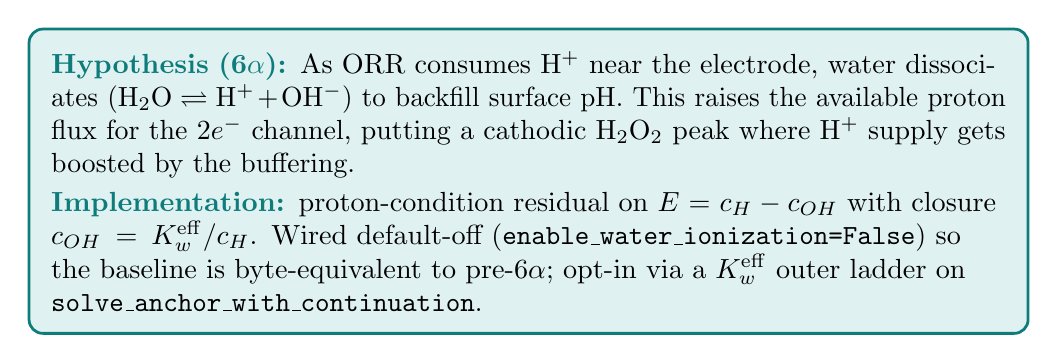
\begin{tikzpicture}[every node/.style={align=left}]
\node[callout={phaseA}{phaseABg}, text width=\textwidth] {%
  \textcolor{phaseA}{\textbf{Hypothesis (6$\alpha$):}} As ORR
  consumes H$^+$ near the electrode, water dissociates
  ($\mathrm{H_2O} \rightleftharpoons \mathrm{H^+} + \mathrm{OH^-}$)
  to backfill surface pH.  This raises the available proton flux for
  the 2$e^-$ channel, putting a cathodic H$_2$O$_2$ peak where H$^+$
  supply gets boosted by the buffering.\\[2pt]
  \textcolor{phaseA}{\textbf{Implementation:}} proton-condition
  residual on $E = c_H - c_{OH}$ with closure
  $c_{OH} = K_w^{\mathrm{eff}}/c_H$.  Wired default-off
  (\texttt{enable\_water\_ionization=False}) so the baseline is
  byte-equivalent to pre-6$\alpha$; opt-in via a $K_w^{\mathrm{eff}}$
  outer ladder on \texttt{solve\_anchor\_with\_continuation}.
};
\end{tikzpicture}

The Phase 6$\alpha$ $L_{\mathrm{eff}}$ transport sweep (8 boundary
thicknesses $\times$ 13 voltage points, $\sim$58~min) converged
cleanly.  Three falsification gates:

\begin{itemize}\setlength{\itemsep}{1pt}
\item[\textbf{P1}] \textcolor{success}{\textbf{PASS}} ---
  Levich linearity preserved across $L_{\mathrm{eff}}$.
\item[\textbf{P2}] \textcolor{success}{\textbf{PASS}} ---
  no spurious cathodic peak introduced.
\item[\textbf{P3}] \textcolor{verdict}{\textbf{FAIL}} ---
  max surface pH was $10.58$ at $L_{\mathrm{eff}}=16~\mu$m, and the
  surface pH was \emph{invariant} with $L_{\mathrm{eff}}$.  A
  textbook bulk water-dissociation rate estimate
  ($\sim$1.4~mol/m$^3$/s) is $\sim$20$\times$ slower than the
  cathodic H$^+$ demand the model needs to sustain.
\end{itemize}

Water does autoionize, but it's \textbf{sub-leading} as a buffer at
deck conditions.  Phase 6$\alpha$ retired as the primary mechanism;
plumbing preserved as opt-in.

%==============================================================
\section{Phase 6$\beta$ --- cation hydrolysis at the OHP}
%==============================================================

The pivot followed the group's own published framing
(Linsey 2025 ACS-CATL deck, Co-Zhang 2019 \emph{Angewandte},
Singh et al.\ 2016 \emph{JACS}).  The proposed mechanism:

\begin{center}
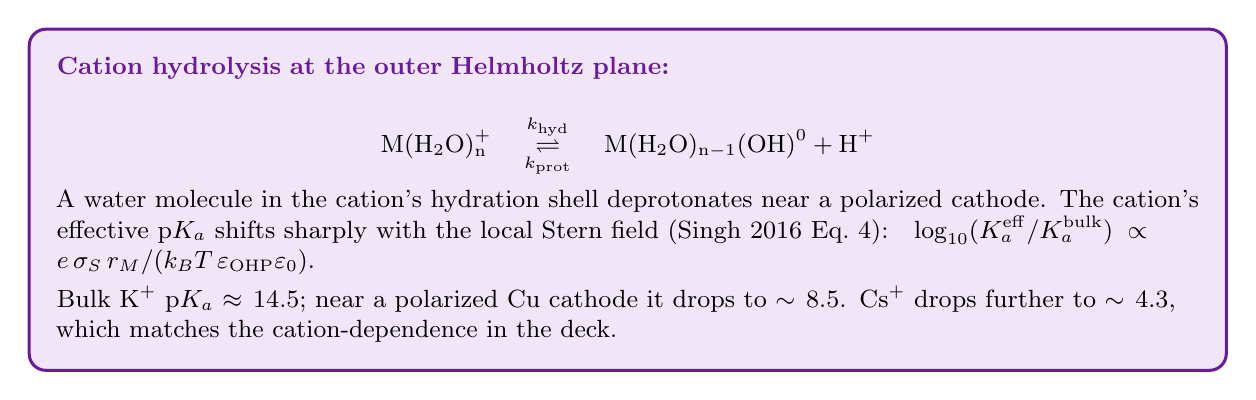
\begin{tikzpicture}

\node[bigbox, draw=phaseB, fill=phaseBBg, text width=14.5cm, font=\small] {%
  \textcolor{phaseB}{\textbf{Cation hydrolysis at the outer Helmholtz plane:}}\\[3pt]
  \[
    \mathrm{M(H_2O)_n^+} \quad
    \underset{k_{\mathrm{prot}}}{\overset{k_{\mathrm{hyd}}}{\rightleftharpoons}} \quad
    \mathrm{M(H_2O)_{n-1}(OH)^0} + \mathrm{H^+}
  \]
  A water molecule in the cation's hydration shell deprotonates near
  a polarized cathode.  The cation's effective p$K_a$ shifts sharply
  with the local Stern field (Singh 2016 Eq.~4):\quad
  $\log_{10}(K_a^{\mathrm{eff}}/K_a^{\mathrm{bulk}})
   \propto e\,\sigma_S\,r_M / (k_BT\,\varepsilon_{\mathrm{OHP}}\varepsilon_0)$.\\[3pt]
  Bulk K$^+$ p$K_a$ $\approx 14.5$; near a polarized Cu cathode it
  drops to $\sim 8.5$.  Cs$^+$ drops further to $\sim 4.3$, which
  matches the cation-dependence in the deck.
};

\end{tikzpicture}
\end{center}

The mechanism is attractive because it's cation-specific: K$^+$, Cs$^+$,
Na$^+$, Li$^+$ each have their own bulk p$K_a$ and Singh shift, and
the deck's cation series should fall out from one set of equations.

%==============================================================
\section{Architecture (v9) and sub-step chronology}
%==============================================================

The v9 architecture (approved after a five-round GPT critique) made
these choices:

\begin{itemize}\setlength{\itemsep}{1pt}
\item \textbf{Dynamic K$^+$.}  K$^+$ becomes a fourth Nernst--Planck
  species (4-DOF stack: O$_2$, H$_2$O$_2$, H$^+$, K$^+$).  No analytic
  Boltzmann counterion for K$^+$ --- the hydrolysis reaction couples
  through K$^+$'s spatial profile, which has to be a real DOF.
\item \textbf{Global $\Gamma_{\mathrm{MOH}}$ on the electrode.}  Surface
  MOH coverage is a single scalar Real-element function on the
  electrode boundary (mol/m$^2$), evolved by finite-rate kinetics.
\item \textbf{Finite-rate kinetics + Langmuir cap.}
  $R_{\mathrm{net}} = k_{\mathrm{hyd}}\,c_{M^+}(0)\,(1 - \Gamma/\Gamma_{\mathrm{max}})
   - k_{\mathrm{prot}}\,c_H(0)\,\Gamma/\delta_{\mathrm{OHP}}$;
  desorption removal $R_{\mathrm{des}} = k_{\mathrm{des}}\,\Gamma$
  treated as an open reservoir.
\item \textbf{No Stern surface-charge correction.}  Cation hydrolysis
  couples to Poisson purely through dynamic $c_{K^+}$; no separate
  surface-charge bookkeeping.
\end{itemize}

Sub-steps after v9, in chronological order:

{\footnotesize
\renewcommand{\arraystretch}{1.25}
\begin{longtable}{@{}>{\raggedright\arraybackslash}p{2.0cm}%
                    >{\raggedright\arraybackslash}p{6.0cm}%
                    >{\raggedright\arraybackslash}p{5.7cm}@{}}
\toprule
\textbf{Step} & \textbf{What changed} & \textbf{Outcome} \\
\midrule
\endhead

\textbf{v10a} &
  Langmuir cap $(1-\Gamma/\Gamma_{\mathrm{max}})$ on the hydrolysis
  rate; $\Gamma_{\mathrm{max}} \approx 0.047$ nondim
  ($\approx$ one monolayer of hydrated MOH at the OHP). &
  Closed-form Picard converges; saturation behaves smoothly. \\
\addlinespace

\textbf{v10a$'$} V-sweep &
  $C_S = 0.20$~F/m$^2$ (Bohra-Koper-Choi consensus) and
  $K_0^{R4e}$ factor $= 10^{-14}$ to probe 2$e^-$/4$e^-$ coexistence;
  V-sweep across the deck band. &
  V$_{\mathrm{kin}} = -0.10$~V passes the primary route
  ($\sigma_S {<} 0$, branch active, not transport-artifact, not
  cap-dominated); K$^+$ enrichment dominates $F_0$ cathodically. \\
\addlinespace

\textbf{A.2}
  $k_{\mathrm{hyd}}$ grid &
  10-rung $k_{\mathrm{hyd}}$ ladder at V$_{\mathrm{kin}}$,
  $\lambda{=}1.0$. &
  10/10 rungs converge, mass-balance at machine precision;
  selectivity gap at V$_{\mathrm{kin}}$ is only $+5$~pp, so
  $\Gamma_{\mathrm{max}}$ / $k_{\mathrm{des}}$ retune flagged
  \emph{low priority}. \\
\addlinespace

\textbf{Step 6} plumbing &
  Four wiring paths verified
  (form-build residual, p$K_a$-shift context, Picard $\Gamma$ update,
  diagnostics) via ablation. &
  All pass; physics finding: K$^+$ Boltzmann pile-up
  ($c_K \approx 291$ nondim at OHP) makes a 5\,\% sentinel floor
  unreachable below $R_{\mathrm{inj}} \leq 10$. \\
\addlinespace

\textbf{v10b} calibration &
  Literature-grounded lock of three parameters:
  $\Gamma_{\mathrm{max}}{=}0.047$,
  $k_{\mathrm{des}}{=}1.0$ (Eyring prior $\Delta G \approx 0.80$~eV),
  $C_S{=}0.20$~F/m$^2$.
  Sensitivity sweeps D7-D1 (C$_S$ bracket) and D7-D4 (3$\times$5$\times$2
  matrix). &
  All hard gates pass (cd${<}0$, R$_{4e}$ sign preserved,
  $R_{\mathrm{net}}\geq 0$, mass-balance rel $\leq 5{\times}10^{-3}$). \\
\addlinespace

\textbf{Step 9} B.2 &
  Densified 14$\times$10 $= 140$-rung
  $k_{\mathrm{hyd}}{\times}\lambda$ grid at V$_{\mathrm{kin}}$. &
  14/14 $k_{\mathrm{hyd}}$ converge at $\lambda{=}1$
  (after step 9.5 added \texttt{warm\_start\_floor} bisection for
  $\lambda{=}0$ rungs);
  mass-balance $\leq 5{\times}10^{-13}$. \\
\addlinespace

\textbf{Step 10} Phase D &
  Fit a single scalar $\Delta_\beta$
  (carbon-vs-Cu offset in Singh Eq.~4) against the deck K$_2$SO$_4$
  H$_2$O$_2$ selectivity at pH 3.5--4.5
  (deck mean $50.95$\,pp).  Two paths tested:
  Stern $\sigma$-mapping and ablation $\sigma$-override. &
  \textcolor{verdict}{\textbf{OUTCOME\_C\_NON\_IDENTIFIABLE\_flagged}}
  --- $\Delta_\beta$ alone cannot match the deck.  See callout below. \\

\bottomrule
\end{longtable}
}

%==============================================================
\section{Current state --- the Phase D verdict}
%==============================================================

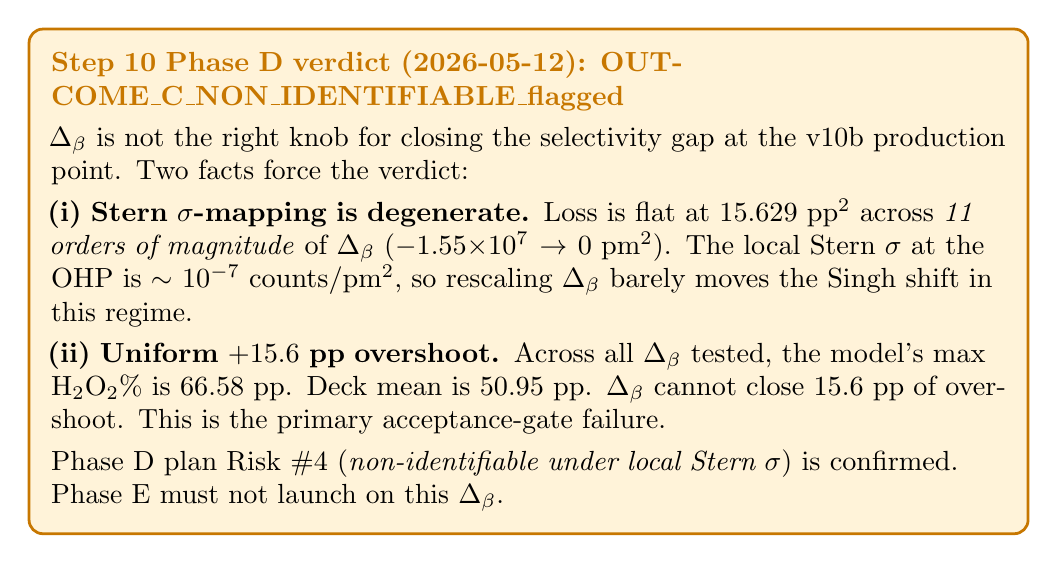
\begin{tikzpicture}
\node[callout={verdict}{verdictBg}, text width=\textwidth] {%
  \textcolor{verdict}{\textbf{Step 10 Phase D verdict
    (2026-05-12): OUTCOME\_C\_NON\_IDENTIFIABLE\_flagged}}\\[3pt]
  $\Delta_\beta$ is not the right knob for closing the selectivity
  gap at the v10b production point.  Two facts force the
  verdict:\\[3pt]
  \textbf{(i) Stern $\sigma$-mapping is degenerate.}
  Loss is flat at $15.629$~pp$^2$ across \emph{11 orders of magnitude}
  of $\Delta_\beta$
  ($-1.55{\times}10^7 \to 0$~pm$^2$).  The local Stern $\sigma$ at the
  OHP is $\sim 10^{-7}$ counts/pm$^2$, so rescaling $\Delta_\beta$
  barely moves the Singh shift in this regime.\\[3pt]
  \textbf{(ii) Uniform $+15.6$~pp overshoot.}
  Across all $\Delta_\beta$ tested, the model's max H$_2$O$_2$\% is
  $66.58$~pp.  Deck mean is $50.95$~pp.  $\Delta_\beta$ cannot close
  $15.6$~pp of overshoot.  This is the primary acceptance-gate
  failure.\\[3pt]
  Phase D plan Risk \#4 (\emph{non-identifiable under local Stern
  $\sigma$}) is confirmed.  Phase~E must not launch on this
  $\Delta_\beta$.
};
\end{tikzpicture}

%==============================================================
\section{Open issues and what's blocked}
%==============================================================

\begin{enumerate}\setlength{\itemsep}{2pt}

\item \textbf{Steric coefficient discrepancy for dynamic species}
  (surfaced 2026-05-12 during Phase D bridge diagnostics).
  O$_2$, H$_2$O$_2$, H$^+$ are all seeded with
  \fname{A_DEFAULT = 0.01}, which corresponds to a hard-sphere radius
  $r \approx 14.9$~\AA\ ---  $\sim$150$\times$ larger than the physical
  values
  (O$_2$ r=1.7~\AA, H$_2$O$_2$ r=2.0~\AA, H$^+$ r=2.8~\AA\ for
  H$_3$O$^+$ Stokes).  H$^+$ in particular is therefore clamped
  $\sim$150$\times$ tighter than its real Bikerman cap would allow.
  The Phase D \emph{non-identifiability} verdict is independent of
  this, but the $+15.6$~pp overshoot might not be ---
  \emph{anything that depends on the Levich plateau setting H$^+$
  supply is suspect until the physical-$a$ bridge runs land.}

\item \textbf{$\Delta_\beta$ cannot close the gap alone.}
  Phase~D$'$ / Phase~6$\gamma$ candidate scopes (in rough order of
  likelihood):
  \begin{itemize}\setlength{\itemsep}{1pt}
    \item Re-fit $k_{\mathrm{des}}$ and $\Gamma_{\mathrm{max}}$ (Phase D
      locked these as v10b-calibrated; falsification re-opens them).
    \item $r_{\mathrm{H,El}}$ sensitivity sweep --- the Cu prior
      ($200.98$~pm) may not transfer cleanly to CMK-3 carbon.
    \item Local-pH / mass-transport coupling --- model selectivity is
      V-flat, which suggests it's transport-limited and the H$^+$
      Levich convention may need re-examination.
    \item Singh formula \emph{structure} (Plan §3.1 locked the form as
      a hard invariant; if $\Delta_\beta$-alone fails the structure
      may itself need revisit --- this is a bigger paradigm change).
  \end{itemize}

\item \textbf{Phase~6$\delta$ (parallel alkaline ORR kinetics) likely
  still needed.}  Cation hydrolysis fixes the local-pH \emph{source},
  not the downstream decay mechanism.  If 6$\beta$ only ever produces
  a plateau, 6$\delta$.1 (explicit $R_{\mathrm{2e,alk}}$ +
  $R_{\mathrm{4e,alk}}$ parallel reactions) would be the next step ---
  the order is then 6$\beta$.1 $\to$ measure $\to$ 6$\delta$.1
  $\to$ measure.

\item \textbf{Singh 2016 SI extraction.}  Phase D used a placeholder
  $\Delta\mathrm{p}K_a = \beta_M\,\mathrm{sgn}(\sigma_S)\,|\sigma_S|^p$
  with $p \in \{0.5, 1.0, 2.0\}$.  A clean re-read of the Singh SI
  for the exact functional form (sign, $\ln 10$ factor, distance
  dependence) is queued.

\item \textbf{Cation-series transferability (Phase~E).}  $\beta$
  values from Singh 2016 are CO$_2$RR-on-Cu; transferability to
  ORR-on-carbon is an assumption.  Phase~E is a \emph{predictive
  screen}, not a decisive falsifier --- if the (Cs, Na, Li) holdout
  fails, audit the Stern/OHP field mapping before rejecting the
  cation-hydrolysis hypothesis outright.

\end{enumerate}

%==============================================================
\section*{Net summary}
%==============================================================

What landed cleanly: the architecture (v9 dynamic K$^+$ +
$\Gamma_{\mathrm{MOH}}$ + finite-rate kinetics), the literature
calibration (v10b $\Gamma_{\mathrm{max}}$, $k_{\mathrm{des}}$,
$C_S$), and all the plumbing (step 6, step 9, step 9.5 floor
bisection).  All convergence and mass-balance gates pass.

What didn't land: the \emph{fit}.  $\Delta_\beta$ degeneracy at the
production Stern $\sigma$ means the parameter Plan D was built around
can't pull selectivity down by the needed $\sim$15.6~pp.

What's holding things up: (a)~the steric-coefficient bridge runs
disambiguating whether the H$^+$ Bikerman clamp is silently
producing the overshoot, and (b)~a decision on whether to open
$k_{\mathrm{des}}$/$\Gamma_{\mathrm{max}}$ as additional fit
parameters or revisit the Singh formula structure itself.  Until
(a) and (b) resolve, Phase~E remains blocked.

\vspace{1em}
\noindent\textbf{See also:}
\begin{itemize}\setlength{\itemsep}{1pt}\small
\item \texttt{docs/phase6/PHASE\_6A\_INVESTIGATION\_SUMMARY.md} ---
  Phase~6$\alpha$ outcome + Phase~6$\beta$ scoping handoff.
\item \texttt{docs/phase6/phase6b\_next\_steps\_plan.md} ---
  live Phase~6$\beta$ plan.
\item \texttt{docs/phase6/phase6b\_step10\_phase\_D\_summary.md} ---
  Step 10 Phase D detailed writeup.
\item \texttt{docs/phase6/v10b\_calibration\_summary.md} ---
  v10b $\Gamma_{\mathrm{max}}$ / $k_{\mathrm{des}}$ / $C_S$ literature
  grounding.
\item \texttt{docs/phase6/CONJECTURE\_AUDIT\_2026-05-09.md} ---
  Cs$^+$ vs deck-baseline K$^+$ audit.
\item Companion writeup
  \emph{Forward Solver Codepath}
  (\texttt{forward\_codepath\_demo\_slide15.pdf}, this directory) ---
  what the solver \emph{does} converge cleanly when 6$\alpha$ /
  6$\beta$ are off (default-off byte-equivalent baseline).
\end{itemize}

\end{document}
